
\documentclass [11pt]{article}
\usepackage{graphicx}

\title{Pastured Poultry Egg Project}
\author{Carl Chandler, PhD \\Sun Aquasystems and Chandler Family Farm}

\begin{document}
\maketitle

\section{Introduction}
This is a project to document all the necessary parts for raising layer hens on pasture, and trying to optimize for profitability. It is not a strictly scientific paper, more a review of literature and a documentation of all the little details that are important for either raising pastured poultry for profit or experimental design involving pastured poultry. Small flocks of hens are often kept in rural Nova Scotia, free-range or small runs, and the eggs are marketed on roadside stands, usually using a cooler and the honour system for self-serve sales. These eggs are perceived to be healthier and, in fact, may be higher in vitamins and omega-3s \cite{karsten2010vitamins}.  Profitability is generally not a concern as most producers keep the birds as a hobby; however, I believe there is potential for a profitable enterprise. There are many online blogs and even some scientific papers on pastured laying hens. However, many of these assume that the reader is already a chicken farmer or is only keeping them for a hobby. Others give the basic idea, but leave the reader to work out the details. \cite{berton2012} My objective here is a detailed explanation of what is needed to start up a pastured layer operation, common pitfalls or at least errors that I've made. Finally, I will try to keep advice based on real experiments and published research instead of arguing from "it worked for me, so it's the best" style rhetoric. This is also an evolving document, supplemented by the rest of the files in this Git directory. I aim to document a more profitable method of raising poultry, following the results of my own trials and experiments.  

There are two basic methods for raising chickens in pasture.\cite{clancy2006} You can have a mobile house for the birds to roost in at night and a portable fence around that. This is moved through the field manually once a week-ish. The second is to keep the birds in a tractor with walls and roof of at least mesh but no floor. They have access to that patch of field, and it's moved every day. There are a few other options, a permanent coop and fields around it that are rotated through, many tiny coops spread over a large field. The need for fresh ground is key, chickens will rapidly destroy any plant/sod if the land is not given a chance to recuperate. What the critical stocking density / rotational interval is not well established. British free-range egg producers require 1 acre of run for 1000 birds \cite{britishFreeRangEegg}, Australian regulations require no more than 10000 hens per hectare, but 1500 birds per hectare is seen as best practice \cite{animalsAustralia}. Some advocate for no more than 50 birds per acre, which was considered best practice before modern fertilizers, 50 birds being potentially over fertilizing the field for grain. [6] Very low stocking density seems to require movable shelters. 10000 hens per hectare is one bird per m2 which will assuredly kill all plant life. 

Profitability means keeping input costs low. The sale price is generally fixed by the going rate in grocery stores for direct marketing, though depending on the market a pasture raised egg can sell for a premium over an egg from a large scale indoor layer egg farm. The vast majority of the cost is feed and labour, but capital for coops, washing eggs, buying/hatching hens, and marketing also plays a role.


\section{Equipment and Capital}
talk about equipment for each system. Put in cad drawings, save cad files and upload parasolids, also put onshape link. Also put in pictures of my setups. Talk about failed methods- skids no, small wheels no, winches no. tractor... can't imagine that it helps, esp when ground is soft from rain. 
\subsection{2025 jan as built}
\begin{figure}
    \centering
    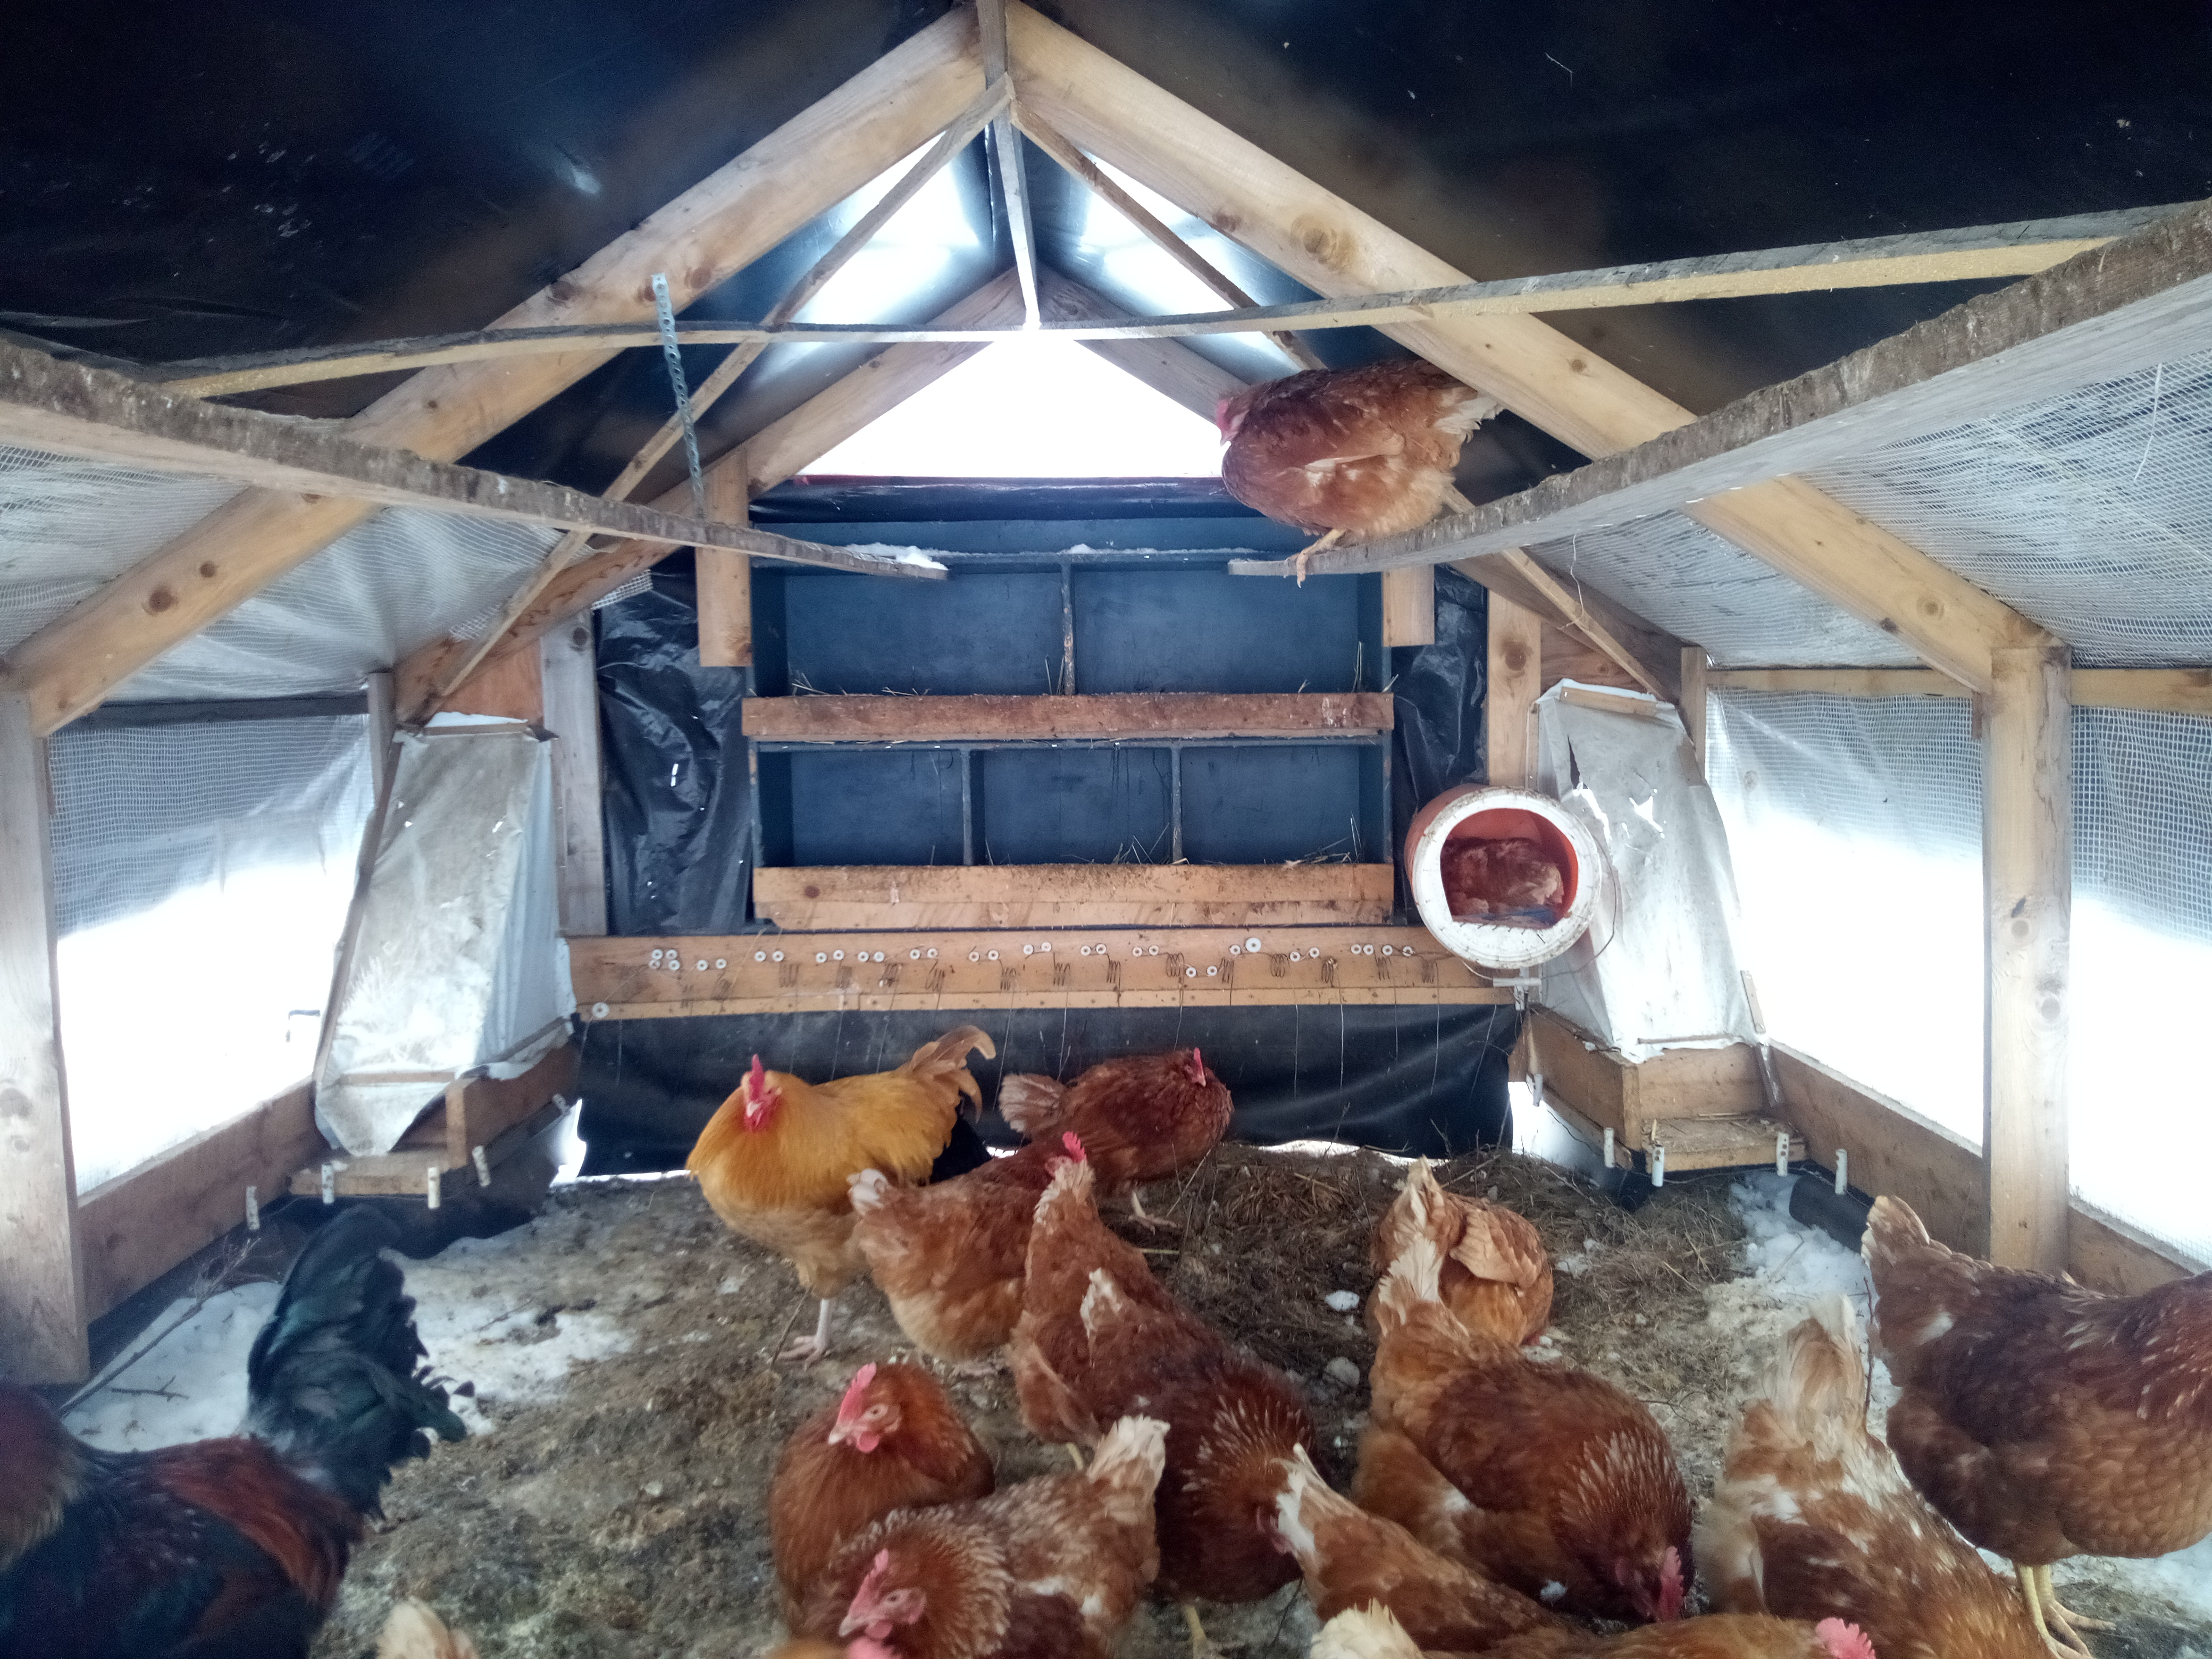
\includegraphics[width=0.75\linewidth]{inside_coop.jpg}
    \caption{Inside chicken tractor 16 jan 2025}
    \label{fig:enter-label}
\end{figure}

\section{Common problems }
rats
fence tangles
electric fence shorts 
snow 
wind 
mud 

\section{Winter}
talk about winter- in my mind this is an unsolved problem. feed consumption 1.5 times summer rate in unheated coop. Can you save money with an indoor setting for winter? 

\section{Cost breakdown}
This section refers to the included spreadsheet 

\section{ Egg washing}
I wash eggs by hand. THey also need to by dried before putting into cartons or they can stick and then break when the customer tries to remove them. An egg washing machine would be nice, but it would have to be quite cheap. 
\url{https://thelittleeggscrubber.com/} looks interesting but still kind of expensive, esp in CAD

\Section{ Marketing}
I have been using the cooler and honour system. I have a locked money box where people can insert bill and coins, I also have posted information for e-transfer. E-transfer is not super popular but it is used occasionally. A cooler with ice works fine in the summer; in below-zero weather, I include a 4l jug of 20c water in the beginning of the day and this seems to prevent the eggs from freezing. I have a roadside stand in a rural but reasonably high traffic area. Most customers buy 1-2 dozen at a time. I have a few customers that buy 4-8 dozen eggs at a time, albeit infrequently. Competition from hobby farm egg sellers is minimal in the winter because hobby farmers typically do not supply supplemental lighting in the winter, and thus have very few eggs. Snow and poor weather does seem to mean fewer people stopping to buy eggs. Most customers are good about returning cardboard egg cartons for reuse, I've never had to buy cartons. 






\bibliographystyle{IEEEannot}
\bibliography{pasturedpoultrybib}
\end{document}